\chapter{Notes}

\todo[inline]{Remove Notes before releasing.}

% ------------------------------------------------------------------------------
\section{Weighted Sum MKN Algorithm from Code}

\begin{algorithm}
  \caption{Weighted Sum MKN algo from Code (likely optimizable)}
  \begin{algorithmic}[1]
    \Require $h$
      \Comment{History for which to determinate interpolation weights}
    \Ensure $\SumWeight_i^h$
      \Comment{Array of interpolation weights}

    \LineComment{Find first seen history $\SeenHistory$}
    \State $\SeenHistory \gets h$
    \While{$\Count(\SeenHistory \Skp) = 0$}
      \State $\SeenHistory \gets \SeenHistory\text{.backoff()}$
             \todo[inline]{Better notation for backoff}
    \EndWhile
    \State $N = \StringLength{\SeenHistory} + 1$
    \State $\SumWeight^h \gets$ new array of size $N$
    %\State
    \State $nominator \gets 1$
    \State $denominator \gets \Count(\SeenHistory \Skp)$
    \State $\SumWeight_1^h \gets \frac{1}{denominator}$
    %\State
    \State $\History \gets \SeenHistory$
    \For{$i \gets 2, N$}
      \State $nominator \gets \gamma(\History) \frac{nominator}{denominator}$
      \State $\History \gets \History\text{.backoff()}$
      \State $denominator \gets \ContCountIp(\WSkp \History \WSkp)$
      \State $\SumWeight_i^h \gets \frac{nominator}{denominator}$
    \EndFor
  \end{algorithmic}
\end{algorithm}

% ------------------------------------------------------------------------------
\clearpage
\section{Alternative Binomial Diamond of order 3}

\begin{figure}[H]
  \centering
  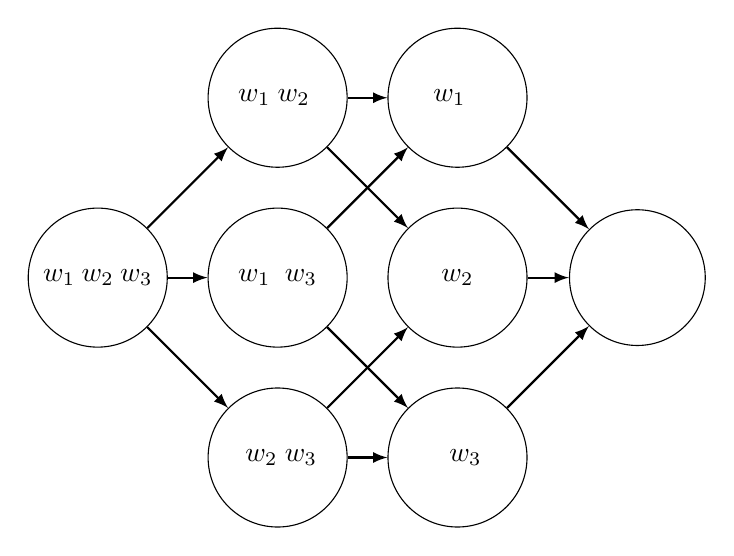
\begin{tikzpicture}[
    node distance = 6.5em,
    seq/.style = {draw, circle, align=center, text centered, text width=4.2em},
  ]
    \node [seq] (000)                {$w_1 \: w_2 \: w_3$};

    \node [seq] (010) [right of=000] {$w_1 \: \Skp \: w_3$};
    \node [seq] (001) [above of=010] {$w_1 \: w_2 \: \Skp$};
    \node [seq] (100) [below of=010] {$\Skp \: w_2 \: w_3$};

    \node [seq] (101) [right of=010] {$\Skp \: w_2 \: \Skp$};
    \node [seq] (011) [above of=101] {$w_1 \: \Skp \: \Skp$};
    \node [seq] (110) [below of=101] {$\Skp \: \Skp \: w_3$};

    \node [seq] (111) [right of=101] {$\Skp \: \Skp \: \Skp$};

    \path[->, >=latex, thick]
      (000) edge (001)
      (000) edge (010)
      (000) edge (100)

      (001) edge (011)
      (001) edge (101)
      (010) edge (011)
      (010) edge (110)
      (100) edge (101)
      (100) edge (110)

      (011) edge (111)
      (101) edge (111)
      (110) edge (111);
  \end{tikzpicture}
\end{figure}

% ------------------------------------------------------------------------------
\begin{landscape}
  \section{Binomial Diamond of order 4}
  \begin{figure}[H]
    \centering
    \scalebox{0.7}{
      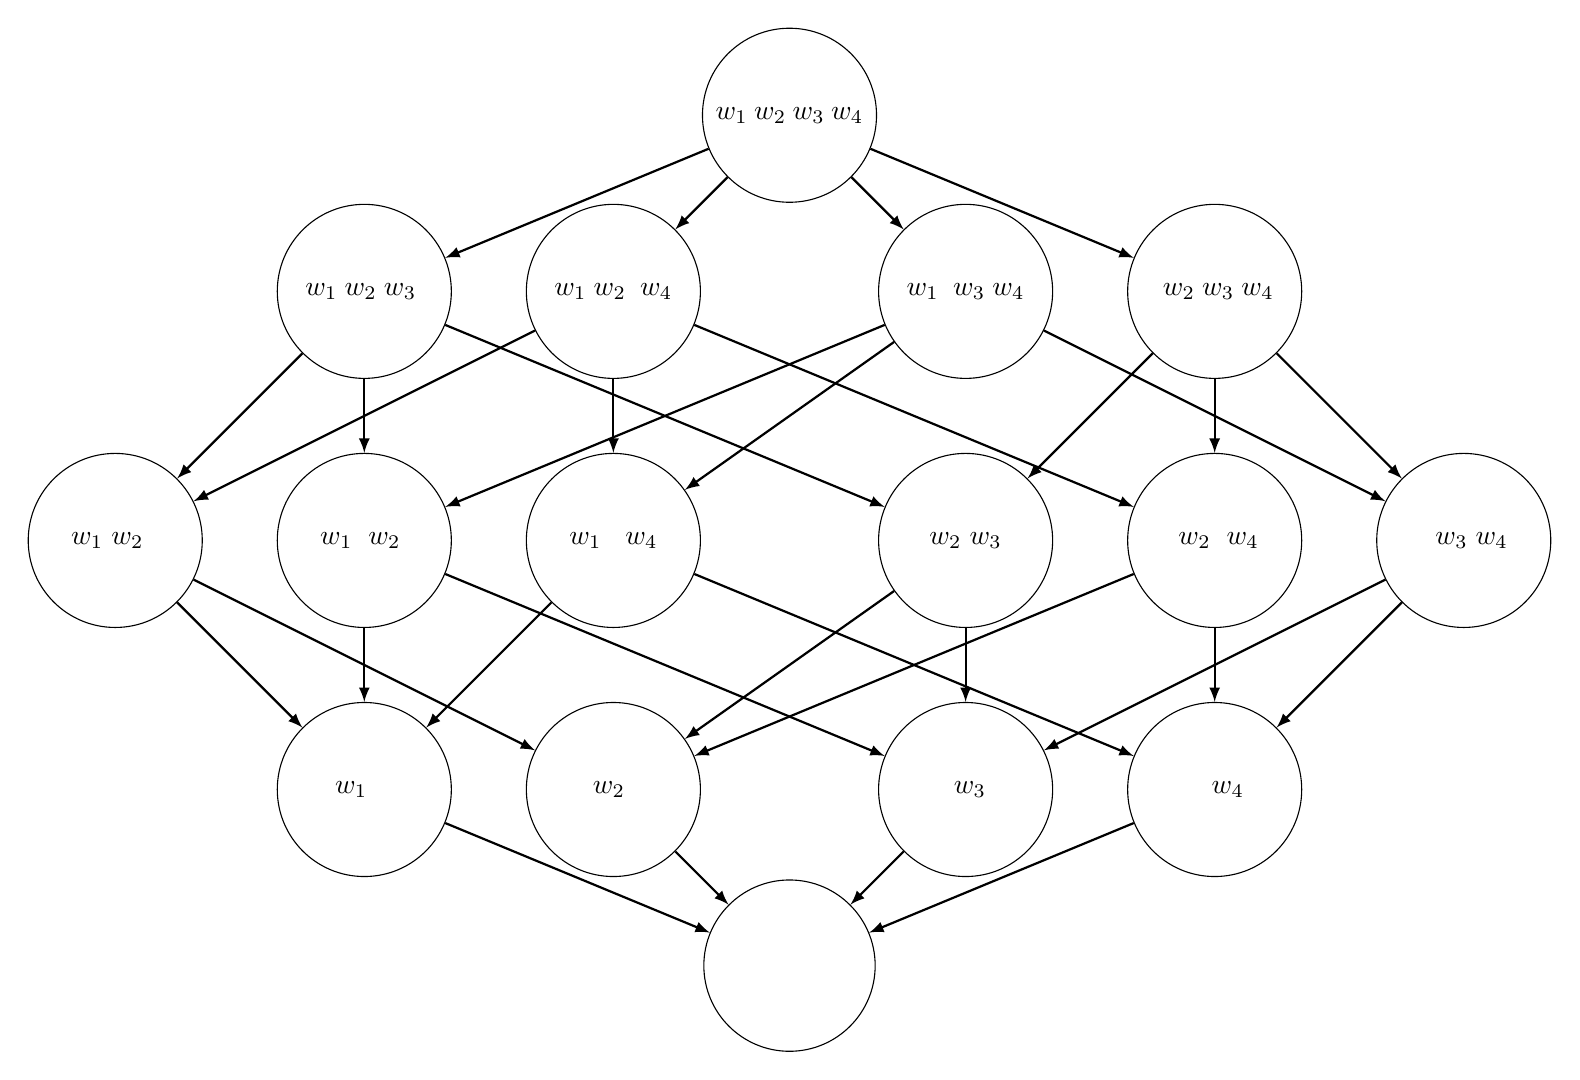
\begin{tikzpicture}[
        node distance = 9em,
        seq/.style = {draw, circle, align=center, text centered, text width=5.5em},
      ]
        \node [seq] (0000) {$w_1 \: w_2 \: w_3 \: w_4$};

        \node [seq] (0010) [below left  of=0000] {$w_1 \: w_2 \: \Skp \: w_4$};
        \node [seq] (0100) [below right of=0000] {$w_1 \: \Skp \: w_3 \: w_4$};
        \node [seq] (0001) [      left  of=0010] {$w_1 \: w_2 \: w_3 \: \Skp$};
        \node [seq] (1000) [      right of=0100] {$\Skp \: w_2 \: w_3 \: w_4$};

        \node [seq] (0101) [below       of=0001] {$w_1 \: \Skp \: w_2 \: \Skp$};
        \node [seq] (0110) [below       of=0010] {$w_1 \: \Skp \: \Skp \: w_4$};
        \node [seq] (1001) [below       of=0100] {$\Skp \: w_2 \: w_3 \: \Skp$};
        \node [seq] (1010) [below       of=1000] {$\Skp \: w_2 \: \Skp \: w_4$};
        \node [seq] (0011) [      left  of=0101] {$w_1 \: w_2 \: \Skp \: \Skp$};
        \node [seq] (1100) [      right of=1010] {$\Skp \: \Skp \: w_3 \: w_4$};

        \node [seq] (0111) [below       of=0101] {$w_1 \: \Skp \: \Skp \: \Skp$};
        \node [seq] (1011) [below       of=0110] {$\Skp \: w_2 \: \Skp \: \Skp$};
        \node [seq] (1101) [below       of=1001] {$\Skp \: \Skp \: w_3 \: \Skp$};
        \node [seq] (1110) [below       of=1010] {$\Skp \: \Skp \: \Skp \: w_4$};

        \node [seq] (1111) [below right of=1011] {$\Skp \: \Skp \: \Skp \: \Skp$};

        \path[->, >=latex, thick]
          (0000) edge (0001)
          (0000) edge (0010)
          (0000) edge (0100)
          (0000) edge (1000)

          (0001) edge (0011)
          (0001) edge (0101)
          (0001) edge (1001)
          (0010) edge (0011)
          (0010) edge (0110)
          (0010) edge (1010)
          (0100) edge (0101)
          (0100) edge (0110)
          (0100) edge (1100)
          (1000) edge (1001)
          (1000) edge (1010)
          (1000) edge (1100)

          (0011) edge (0111)
          (0011) edge (1011)
          (0101) edge (0111)
          (0101) edge (1101)
          (0110) edge (0111)
          (0110) edge (1110)
          (1001) edge (1011)
          (1001) edge (1101)
          (1010) edge (1011)
          (1010) edge (1110)
          (1100) edge (1101)
          (1100) edge (1110)

          (0111) edge (1111)
          (1011) edge (1111)
          (1101) edge (1111)
          (1110) edge (1111);
      \end{tikzpicture}
    }
  \end{figure}
\end{landscape}

% ------------------------------------------------------------------------------
\clearpage
\section{SQL Query Expansion}

\lstset{
  language=SQL,
  emph={token,pattern,pattern1,patternN},
  emphstyle=\textit,
  deletekeywords={count} % Used as column name, don't want to escape it though.
}

\subsection{Modified Kneser Ney Language Model}

\begin{lstlisting}
  SELECT
    token.token AS arg,
    func( 1.count,  11.count, 111.count,
         x1.count, x11.count)
      AS score
  FROM  token
  LEFT OUTER JOIN    1
    ON history(  1) + token =   1.sequence
  LEFT OUTER JOIN   11
    ON history( 11) + token =  11.sequence
  LEFT OUTER JOIN  111
    ON history(111) + token = 111.sequence
  LEFT OUTER JOIN   x1
    ON history( x1) + token =  x1.sequence
  LEFT OUTER JOIN  x11
    ON history(x11) + token = x11.sequence
  ORDER BY score DESC;
  LIMIT k;
\end{lstlisting}

\subsection{Generalized Language Model}

\begin{lstlisting}
  SELECT
    token.token AS arg,
    func( 001.count,  011.count,  101.count, 111.count,
         x001.count, x011.count, x101.count)
      AS score
  SELECT token, score
  FROM token
  LEFT OUTER JOIN  001
    ON history( 001) + token =  001.sequence
  LEFT OUTER JOIN  011
    ON history( 011) + token =  011.sequence
  LEFT OUTER JOIN  101
    ON history( 101) + token =  101.sequence
  LEFT OUTER JOIN  111
    ON history( 111) + token =  111.sequence
  LEFT OUTER JOIN x001
    ON history(x001) + token = x001.sequence
  LEFT OUTER JOIN x011
    ON history(x011) + token = x011.sequence
  LEFT OUTER JOIN x101
    ON history(x101) + token = x101.sequence
  ORDER BY score DESC;
  LIMIT k;
\end{lstlisting}
